% Tipo
\documentclass{article}

% Márgen
\usepackage[margin = 1.5cm]{geometry}

% Símbolos
\usepackage{amsmath}

%Imágenes
\usepackage{graphicx}

%Idioma
\usepackage[spanish]{babel}
\usepackage[utf8]{inputenc}

\begin{document}
    \title{
        Organización y Arquitectura de Computadoras \\
        2019-2 \\
        Práctica 4: Unidad Aritmético Lógica
    }
    \author{
        Sandra del Mar Soto Corderi \\
        Edgar Quiroz Castañeda
    }
    \date{
        3 de marzo del 2019
    }

    \maketitle

    \section{Preguntas}

    \begin{enumerate}
        %1
        \item 
            ¿Qué operaciones aritmeticas y lógicas son básicas para un procesador?
            Justifica tu respuesta.\\
            De operaciones aritmeticas, las básicas son:
            \begin{itemize}
                \item
                Suma: la suma es las operación más importante de todas, ya que 
                se emplea para el cálculo de la dirección de la siguiente 
                instrucción, se utiliza para el cálculo de las direcciones a los 
                operandos y otras operaciones la emplean
                \item
                Resta: Ya que es una de las operaciones aritméticas más 
                importantes, y porque manejamos números inversos
                \item
                Multiplicación: Ya que permite crear después operaciones más 
                complejas
                \item
                División: Es el inverso de la multiplicación
            \end{itemize}

            Para las operaciones lógicas, sería ideal tener un conjunto completo de 
            operaciones. Esto es, las compuertas NAND o NOR, o OR y NOT o NOT y AND. \\
            Sin embargo, para hacer ligeramente más intuitivos los circuitos, 
            se utilizan
            \begin{itemize}
            \item
            AND
            \item
            OR
            \item
            NOT
            \end{itemize}
            Estas 3 son suficientes, pues son completas(podemos expresar 
            cualquier función booleana con ellos).	

        %2		
		\item
        El diseño utilizado para realizar la adición resulta ser ineficiente, 
        ¿Por qué? ¿Qué tipo de sumador resulta ser más eficiente?\\
        Es ineficiente porque tenemos que detectar el caso de uso, un sumador 
        donde el número de sumas y resta esta asociado a las transiciones de 
        ceros y unos, se puede demostrar que resulta en un método más eficiente, 
        pues el número promedio de estas transiciones es menor que el número 
        promedio de unos presentes en una palabra.
		
	
%3	
		\item
		Bajo este diseño, en la ALU se calculan todas las operaciones de forma
        simultanea pero sólo se entrega un resultado, ¿Se realiza trabajo inútil?
        ¿Toma tiempo adicional? ¿Cuál es el costo?\\
        El cálculo de cada operación es (al menos en este diseño) independiente, 
        por lo que cada resultado se calcula en paralelo, por lo que, en general,
        no toma más tiempo calcularlo.\\
        Inclusive, tomaría mayor tiempo y recursos que un sistema determine la 
        operación en particular en lugar de calcular todo.


%4
		\item
        ¿Cuántas operaciones más podemos agregar al diseño de esta ALU? 
        ¿Qué tendríamos que modificar para realizar más operaciones?\\
        Podríamos agregar dos más para tener un total de 8, que son todos los 
        números de 3 bits. Para agregar más funciones, habría que agregar más
        bits de selección de la operación.

        Podríamos agregar multiplicación y división si modificamos partes del 
        circuito y le agregamos circuitos más complejos, como por ejemplo para 
        la multiplicación, necesitariamos agregar un circuito como en la siguiente 
        imagen:
		
		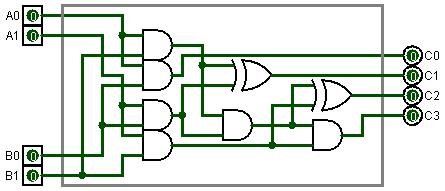
\includegraphics[scale=0.5]{Multiplicador.jpg}
		          
            
    \end{enumerate}
  
    
    
\end{document}